\documentclass[hidelinks, 12pt, oneside]{article}
\usepackage{bookmark}
\usepackage{graphicx}
\usepackage{hyperref}
\usepackage{titlesec}
\setcounter{secnumdepth}{4}
\usepackage[utf8]{inputenc}
\usepackage[english]{babel}


\begin{document}
	\begin{center}
    \centering
    
%University logo
    
\includegraphics[width=144px]{img/icon.png}
    \rule{0\linewidth}{0.15\linewidth}\par
    
    		\begin{center}
		{\uppercase{\Large User Manual\par}}
   		{\Large iCrawler \par}
   			\vspace{1cm} 
   		{\Large Emilio Mumba  \par} 
    		\vspace{1cm}
		   		
    		{\Large The 5 Concurrent Nodes \par} 
    		\vspace{1cm}
		
		{\normalsize Khathutshelo Shaun Matidza\par}
		{\normalsize Sylvester Sandile Mpangane\par}
		{\normalsize Thabang Michael Letageng\par}
		{\normalsize Matthew Nel\par}
		
		\end{center}

		\textbf{}		
		\centering
		\vspace{2cm}
		Department of Computer Science, University of Pretoria

		
	 	{\Large  September 2015}
\end{center}
\clearpage


	\tableofcontents
	
	\newpage
	\section{Vision and Scope}
		\subsection{Project Vision}
		\vspace{0.3 cm}
	  	Digital forensics is defined as the use of scientifically derived and proven methods towards the preservation, 			collection, validation, identification, analysis, interpretation and presentation of digital evidence derived 			from digital sources for the sole purpose of facilitating or furthering the reconstruction of events found to 			be criminal or helping to anticipate the unauthorized actions shown to be disruptive to planned operations.
		Readiness is considered as the process of being prepared for a digital investigation before an incident has 			occurred. \\\\
		The proposal of a mobile monitoring application will promote readiness in digital forensics and protect mobile 			users from malicious entities and activities. It aims to provide a proactive measure that is undertaken by the 		mobile device user or mobile device owner. Having this application installed on mobile devices will proactively 		ensure that relevant digital evidence is made ready and available before an incident occurs. The mobile 				monitoring application is expected to monitor user activities on a mobile device and report application data/logs to a dashboard on a desktop computer. It will generate reports giving the investigator quick and 					comprehensive data/logs that provide a starting point during a mobile device investigation. \newline\newline
		The objective of the mobile monitoring application is to collect data/logs and assist in understanding the 				activities performed by a mobile user as well as shedding more light into the behaviour of the mobile user. 			Combining activities from the various applications promotes a proactive approach which in turn enforces 				proactive (readiness) measures.
		
		\newpage
		\subsection{Project Scope}	
		The high level modules of the iCrawler monitoring app are as indicated in the figure below. Additionally, the responsibilities of each module are noted.
		
			\begin{figure}[!htbp]
    			\centering
    			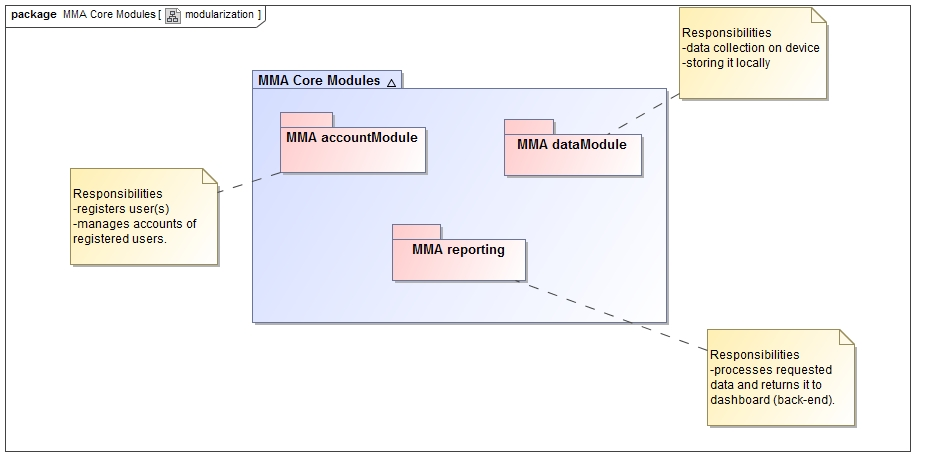
\includegraphics[width=0.9\textwidth]{img/highLevelSystem.jpg}
    			\caption{High Level App Modules}
    			\label{fig:highLevelSystem}
			\end{figure}

	\section{Application Requirements and Design}
	The following section will explain each module in the mobile monitoring app. The use-case design, functional requirements extracted from the use-case along with the selected service contracts will additionally be discussed.\newline
	
	\subsection{Modular System}
	 The application uses a modular design approach. This allows the following to be achieved:
	 \begin{itemize}
	\item add new functionality in the future
 	\item decouple the system
	\end{itemize}


	
	\subsection{iCrawler - Account Module}
	%You will have to elaborate on what the module does (look at the high level module notes for help)
	\subsubsection{Scope}
	%The width and height of the image should not be changed. Just uncomment the line below and specify img source
	
	\begin{figure}[!htbp]
    		\centering
    		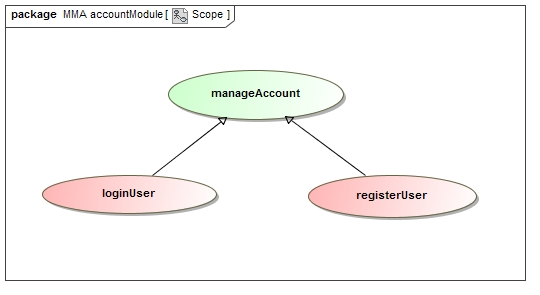
\includegraphics[width=0.9\textwidth]{img/scopeAccounts.jpg}
    		\caption{Scope - mmaAccounts module}
    		\label{fig:accountsScope}
		\end{figure}
		
	\subsubsection{Use-Cases}
		This section provides details on the use-case requirements for the use-cases offered by this module.
	\paragraph{registerUser - priority: important}
		This use-case registers a user on initial installation after user accepts terms and conditions of use.
	
	\newpage
	\subparagraph{Service Contract:}
		The service contract for registerUser is shown in the figure below. The pre-conditions are enforced (raises an exception if not met) and on
		success the user is registered and the device and user data is persisted to the database.
		
		\begin{figure}[!htbp]
    		\centering
    		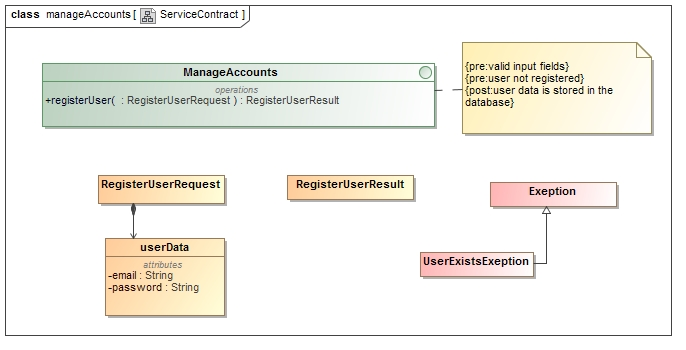
\includegraphics[width=0.9\textwidth]{img/serviceContractRegisterUser.jpg}
    		\caption{Service Contract - Register user}
    		\label{fig:ServiceCon_registerUser}
		\end{figure}
		
		
		\begin{figure}[!htbp]
    		\centering
    		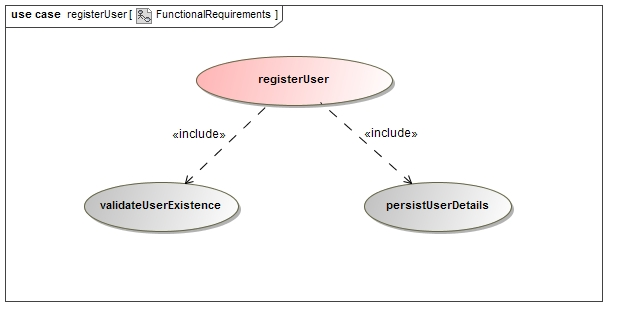
\includegraphics[width=0.9\textwidth]{img/functionalRequirementsRegister.jpg}
    		\caption{Functional Requirements - Register user}
    		\label{fig:FunctionalReq_registerUser}
		\end{figure}
		
		
		
		\paragraph{Process specification:}		
		When a request is made for a user to register, a connection to the database must be established. If no connection to the database can be made, then an exception is thrown. Alternatively, validateUserExistance is called to check if that user exists or not. If the user does exist then an exception is thrown, if not then that user is registered.
		
		\begin{figure}[!htbp]
    		\centering
    		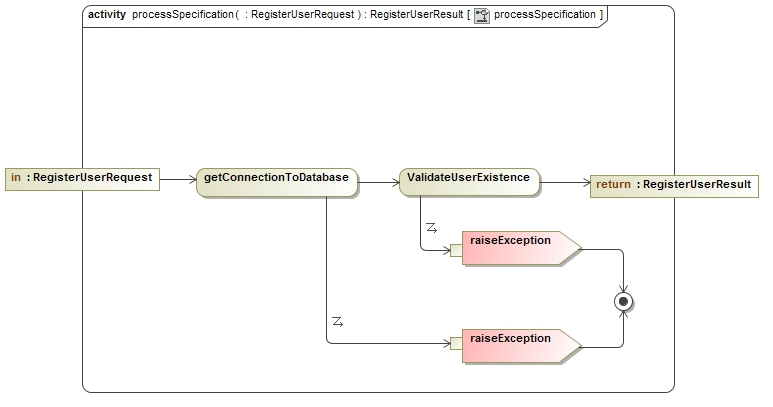
\includegraphics[width=0.9\textwidth]{img/processSpecificationRegisterUser.jpg}
    		\caption{Process Specification - Register user}
    		\label{fig:ProcessSpec_registerUser}
		\end{figure}
				
	
	\paragraph{loginUser - priority: important}
		This use-case logs in a user on initial installation after user accepts terms and conditions of use.
		
	\subparagraph{Service Contract:}
		The service contract for loginUser is shown in the figure below. The pre-conditions that are enforced(raises an exception if not met) and on success the user is logged in and the device, including user data are persisted to the database.\newline 	
	
		\begin{figure}[!htbp]
    		\centering
    		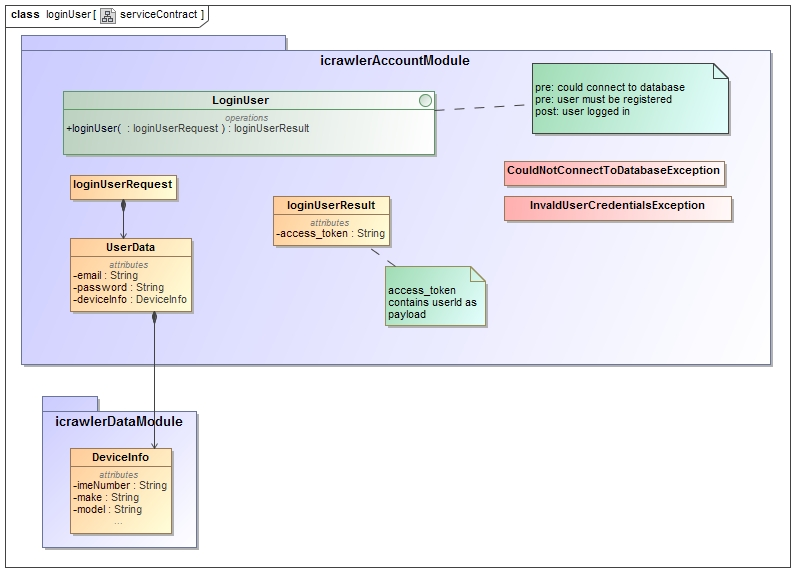
\includegraphics[width=1.0\textwidth]{img/serviceContractLoginUser.jpg}
    		\caption{Service Contract - Login user}
    		\label{fig:ServiceCon_loginUser}
		\end{figure}
		
		
		\begin{figure}[!htbp]
    		\centering
    		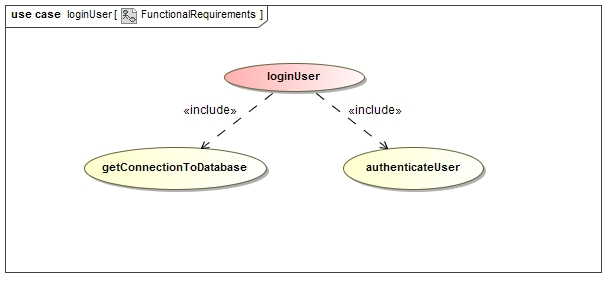
\includegraphics[width=0.9\textwidth]{img/functionalRequirementsLoginUser.jpg}
    		\caption{Functional Requirements - Login user}
    		\label{fig:FunctionalReq_loginUser}
		\end{figure}
		
				
		\newpage
		\paragraph{Process specification:}
		When a request is made for a user to login a connection to the database must be established. If no connection to the database can be made then an exception is thrown. If a connection to the database is established, a login request is made, if user credentials are valid	the user is logged in otherwise an exception is thrown.		
		
		
		\begin{figure}[!htbp]
    		\centering
    		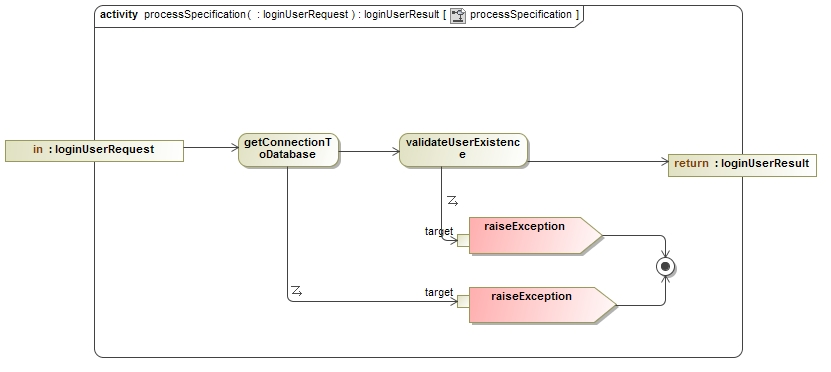
\includegraphics[width=0.9\textwidth]{img/processSpecificationLoginUser.jpg}
    		\caption{Process Specification - Login user}
    		\label{fig:ProcessSpec_loginUser}
		\end{figure}
		\newpage
		
		\subsubsection{Domain Model}
		The domain model for iCrawlerAccountModule.
		
		
		\begin{figure}[!htbp]
    		\centering
    		\includegraphics[width=0.9\textwidth]{img/DomainModelAccountModule.jpg}
    		\caption{Domain Model - Account Module}
    		\label{fig:DomainMod_accountModule}
		\end{figure}
	
	\newpage	
	\subsection{MobileMonitoringApp - Data module}
	%You will have to elaborate on what the module does (look at the high level module notes for help)
	\subsubsection{Scope}
	
		\begin{figure}[!htbp]
    		\centering
    		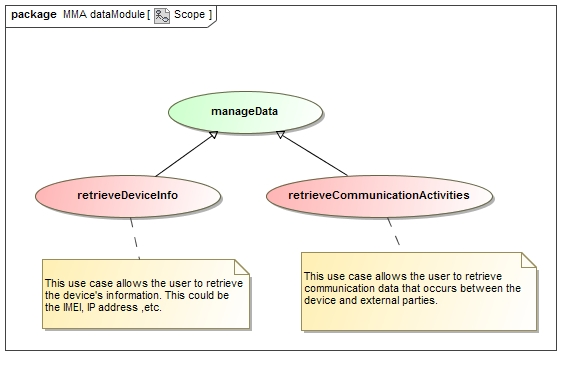
\includegraphics[width=0.9\textwidth]{img/scopeData.jpg}
    		\caption{Scope - dataModule}
    		\label{fig:Scope_dataModule}
		\end{figure}	
		
		
	\subsubsection{Use-Cases}
		This section provides details on the use-case requirements for the use-cases offered by this module.	
		
	\paragraph{retrieveDeviceInfo - priority: important}
		The retrieveDeviceInfo use case retrieves all the relevant device information from the device.\newline
		
		\subparagraph{Service Contract:}
		The service contract for retrieveDeviceInfo is shown in the figure below. The retrieveDeviceInfo 			receives a retrieveDeviceInfoRequest object that specifies the type of data to be retrieved and 			stored locally on to a database.
		
		
		\begin{figure}[!htbp]
    		\centering
    		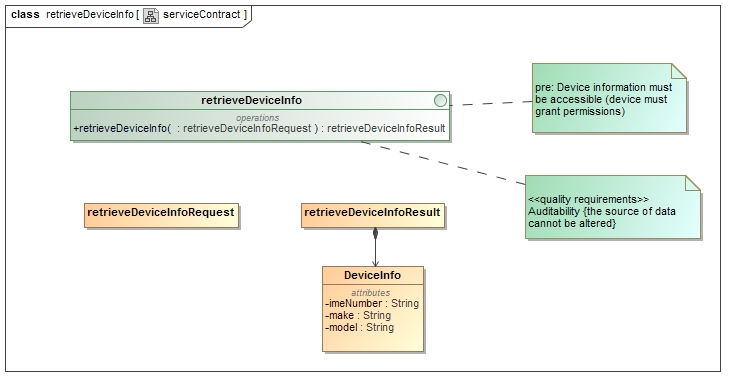
\includegraphics[width=0.9\textwidth]{img/serviceContractRetrieveDeviceInfo.jpg}
    		\caption{Service Contract - retrieveDeviceInfo}
    		\label{fig:ServiceCon_retrieveDeviceInfo}
		\end{figure}


		\begin{figure}[!htbp]
    		\centering
    		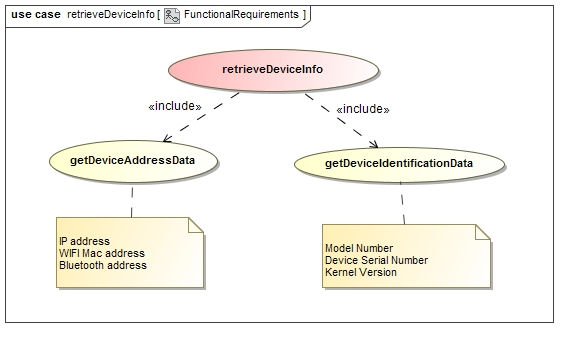
\includegraphics[width=0.9\textwidth]{img/functionalRequirementsRetrieveDeviceInfo.jpg}
    		\caption{Functional Requirements - retrieveDeviceInfo}
    		\label{fig:FunctionalReq_retrieveDeviceInfo}
		\end{figure}
		
		
		\paragraph{Process specification:}
		This activity diagram depicts the process specification for retrieving device information which includes IMEI number, device make and model
		
		\begin{figure}[!htbp]
    		\centering
    		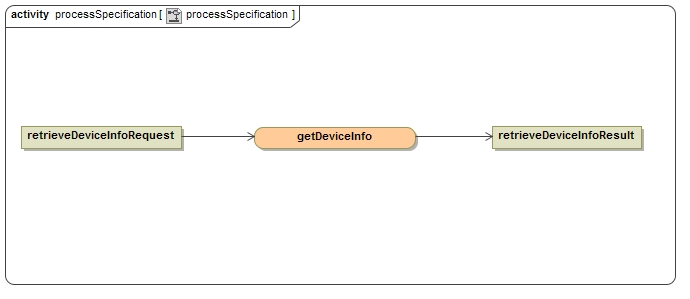
\includegraphics[width=0.9\textwidth]{img/processSpecificationRetrieveDeviceInfo.jpg}
    		\caption{Process Specification - retrieveDeviceInfo}
    		\label{fig:ProcessSpec_retrieveDeviceInfo}
		\end{figure}
		
		
		\paragraph{retrieveLogActivities - priority: important}
		The retrieveLogAcitivites use-case retrieves all the users activity logs from the various apps on the device.\newpage
		
		\subparagraph{Service Contract:}
		The service contract for retrieveLogAcitivites is shown in the figure below. The retrieveLogActivitiesRequest requests the data from the device's content provider and tries to send the data to the server.
		
		\begin{figure}[!htbp]
    		\centering
    		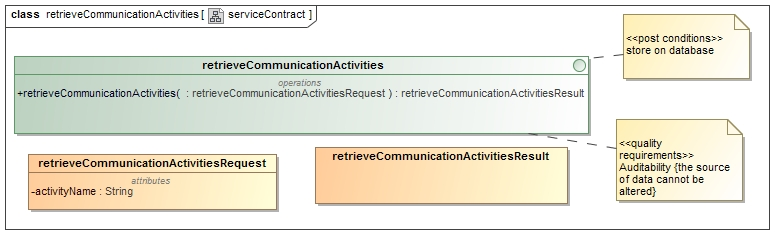
\includegraphics[width=0.9\textwidth]{img/serviceContractRetrieveCommunicationActivities.jpg}
    		\caption{Service Contract - retrieveCommunicationAcitivites}
    		\label{fig:ServiceCon_retrieveCommunicationAcitivites}
		\end{figure}
				

		\begin{figure}[!htbp]
    		\centering
    		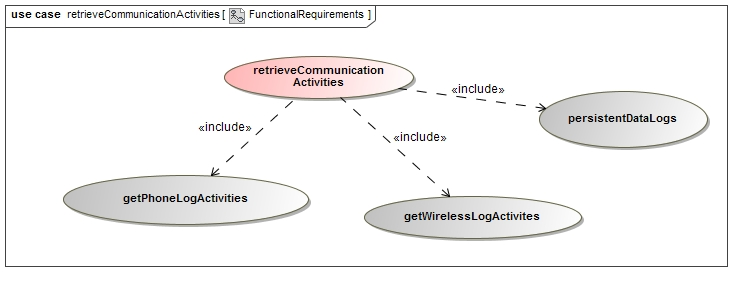
\includegraphics[width=0.9\textwidth]{img/functionalRequirementsRetrieveCommunicationActivities.jpg}
    		\caption{Functional Requirements - Retrieve Communication Acitivites}
    		\label{fig:FunctionalReq_retrieveCommunicationAcitivites}
		\end{figure}	
		
		
			\newpage
			\paragraph{Process specification:}
			The  service receives a request that specifies the type of activity it needs to collect data from. The service will then try to retrieve the data from that activity. Upon retrieving the device logs, the service tries to persist the data logs to the database.
			
			
			\begin{figure}[!htbp]
    		\centering
    		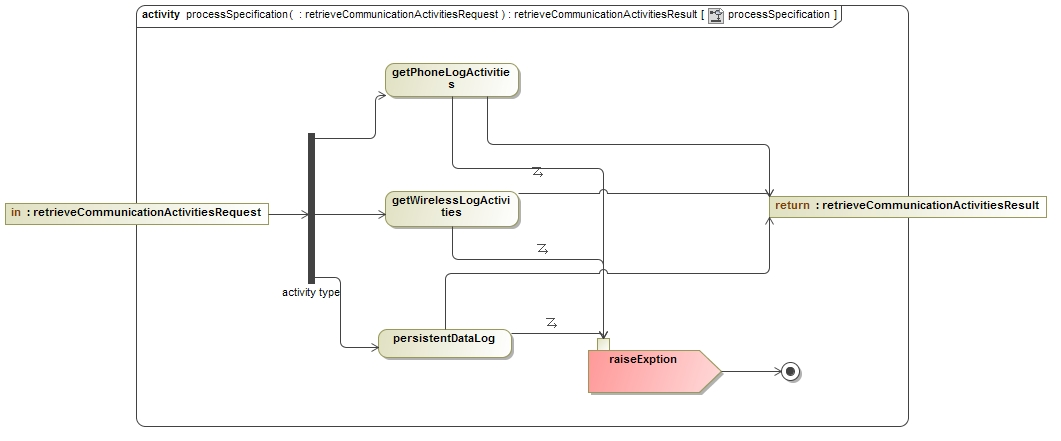
\includegraphics[width=0.9\textwidth]{img/processSpecificationRetrieveCommunicationActivities.jpg}
    		\caption{Process Specification - Retrieve Communication Acitivites}
    		\label{fig:ProcessSpec_retrieveCommunicationAcitivites}
		\end{figure}
		\newpage
	
		\subsubsection{Domain Model}
		The diagram below depicts the domain model for the DataModule .
		
		
		\begin{figure}[!htbp]
    		\centering
    		\includegraphics[width=0.9\textwidth]{img/DomainModelDataModule.jpg}
    		\caption{Domain Model - Data Module}
    		\label{fig:DomainMod_dataModule}
		\end{figure}
		\newpage
		
	\subsection{MobileMonitoringApp - Reports module}
	%You will have to elaborate on what the module does (look at the high level module notes for help)
	\subsubsection{Scope}
	
	
	\begin{figure}[!htbp]
    		\centering
    		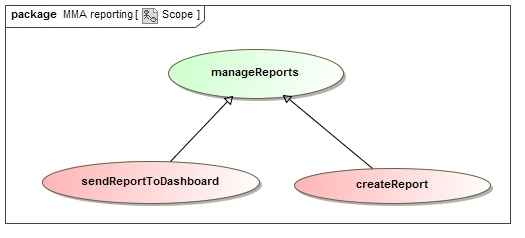
\includegraphics[width=0.9\textwidth]{img/scopeReports.jpg}
    		\caption{Scope - Reporting Module}
    		\label{fig:Scope_reportingModule}
		\end{figure}
			
		
	\subsubsection{Use-Cases}
			This section provides details on the use-case requirements for the use-cases offered by this module.
		\paragraph{ createReport - priority: important}
		This use-case retrieves logs from the device's local database and creates a report from those specific logs.
		\newpage
		
		\subparagraph{Service Contract:}
					The service create report is shown in the figure below. The pre-condition is enforced. 
					
				
		\begin{figure}[!htbp]
    		\centering
    		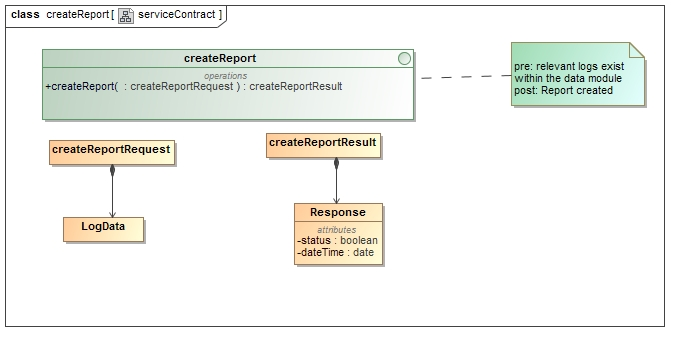
\includegraphics[width=0.9\textwidth]{img/serviceContractcreateReport.jpg}
    		\caption{Service Contract - Create Report}
    		\label{fig:ServiceCon_createReport}
		\end{figure}
		
		
		\begin{figure}[!htbp]
    		\centering
    		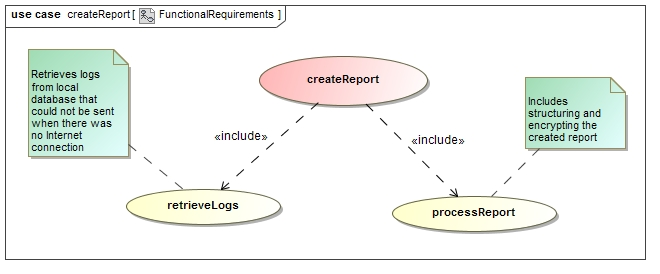
\includegraphics[width=0.9\textwidth]{img/FunctionalRequirementscreateReport.jpg}
    		\caption{Functional Requirements - Create Report}
    		\label{fig:FunctionalReq_createReport}
		\end{figure}
		
		
		\begin{figure}[!htbp]
    		\centering
    		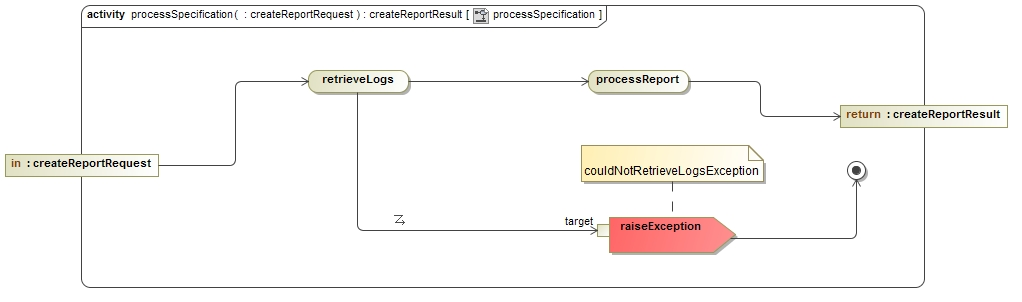
\includegraphics[width=0.9\textwidth]{img/processSpecificationcreateReport.jpg}
    		\caption{Process Specification - Create Report}
    		\label{fig:ProcessSpec_createReport}
		\end{figure}
		\newpage			
					
								
		\paragraph{ sendReportToDashboard - priority: important}
		This module sends the report onto a server where it will be saved on a database to be displayed later on a dashboard .\newline
		\subparagraph{Service Contract:}
			The service contract for sendReportToDashboard is shown in the figure below. The pre-condition is not enforced i.e. If the app fails to establish a connection with the server, the report will be saved temporarily on the device's local database until a connection is established.
			
		
		\begin{figure}[!htbp]
    		\centering
    		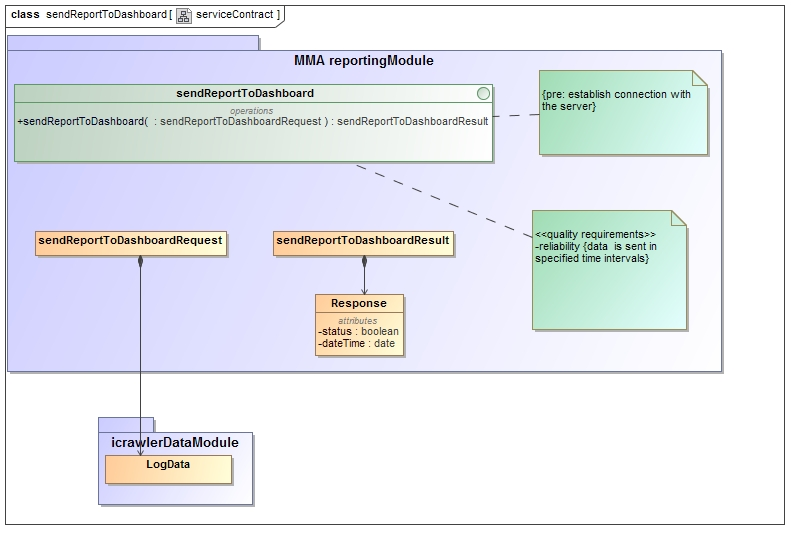
\includegraphics[width=0.9\textwidth]{img/serviceContractSendReportToDashboard.jpg}
    		\caption{Service Contract - Send Report To Dashboard}
    		\label{fig:ServiceCon_submitReport}
		\end{figure}
		\newpage	
			
		\begin{figure}[!htbp]
    		\centering
    		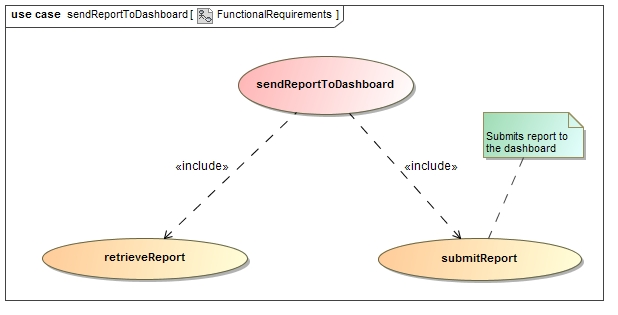
\includegraphics[width=0.9\textwidth]{img/functionalRequirementsSendReportToDashboard.jpg}
    		\caption{Functional Requirements - Send Report To Dashboard}
    		\label{fig:FunctionalReq_submitReport}
		\end{figure}
		
		
		\begin{figure}[!htbp]
    		\centering
    		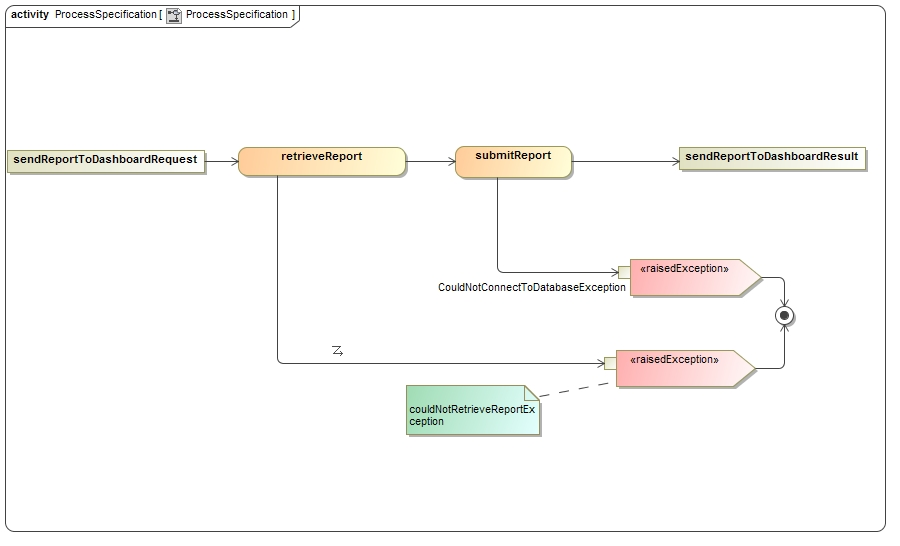
\includegraphics[width=0.9\textwidth]{img/ProcessSpecificationSendResportToDashboard.jpg}
    		\caption{Process Specification - Send Report To Dashboard}
    		\label{fig:ProcessSpec_submitReport}
		\end{figure}
\newpage
\documentclass[hidelinks, 12pt, oneside]{article}
\usepackage{bookmark}
\usepackage{graphicx}
\usepackage{hyperref}
\usepackage{titlesec}
\setcounter{secnumdepth}{4}
\usepackage[utf8]{inputenc}
\usepackage[english]{babel}


\begin{document}

	\begin{center}
    \centering
    
%University logo
    
\includegraphics[width=144px]{img/icon.png}
    \rule{0\linewidth}{0.15\linewidth}\par
    
    		\begin{center}
		{\uppercase{\Large User Manual\par}}
   		{\Large iCrawler \par}
   			\vspace{1cm} 
   		{\Large Emilio Mumba  \par} 
    		\vspace{1cm}
		   		
    		{\Large The 5 Concurrent Nodes \par} 
    		\vspace{1cm}
		
		{\normalsize Khathutshelo Shaun Matidza\par}
		{\normalsize Sylvester Sandile Mpangane\par}
		{\normalsize Thabang Michael Letageng\par}
		{\normalsize Matthew Nel\par}
		
		\end{center}

		\textbf{}		
		\centering
		\vspace{2cm}
		Department of Computer Science, University of Pretoria

		
	 	{\Large  September 2015}
\end{center}
\clearpage


	\tableofcontents
	\newpage
	
	\section{Introduction}
	
	This document contains the software (application) architectural requirements specification which is the infrastructure upon which the application will be developed.\\\\
	The following requirements will be addressed:
	\begin{itemize}
		\item Quality requirements
		\item Architectural Patterns or Styles
		\item Access and Integration Channels
		\item Technologies
	\end{itemize}	 
	\newpage
	\section{Android Application Requirements}
	\subsection{Architectural Requirements}
		\subsubsection{Critical Quality Requirements} 
			\subsubsection*{Auditability}
			\textbf{Description} \\\\
			Auditability refers to the ability to account for a system's usage by the user and be able to monitor events and create logs on what are the user's actions within the system.\\\\
			\textbf{Justification}\\\\
			iCrawler's main functionality is to monitor the user's device activities and report all logs of that particular device.\\\\
			\textbf{Mechanism}
				\begin{enumerate}
					\item Strategy: \\\\
						Auditability can be achieved by:
						\begin{itemize}
							\item Resource Monitoring: A tactic that registers all the events and resources that the application uses; a log of these resource usage is then created.  
						\end{itemize}
					\item Architectural Pattern(s):
						\begin{itemize}
							\item To monitor the application events and resources a design pattern such as the \emph{Observer} pattern can be implemented by the application that can register all events and resource usage. 
						\end{itemize}
				\end{enumerate}	
			\newpage
			\subsubsection*{Security}
				\textbf{Description} \\\\
				Security is the degree of resistance to, or protection from, harm. It applies to any vulnerable and valuable asset, such as a person, dwelling, community, nation, or organization.\\\\
				\textbf{Justification} \\\\
				Security is a critical aspect of any system that deals with critical and confidential data, the strategies used for security provides mechanisms to protect data from unauthorized access and modification. For our mobile monitoring application this means the following:
				\begin{itemize}
					\item No one (person or program) should be able to delete the data collected on device.
					\item When the data is transferred over the network, data should be protected from being intercepted or hacked.    
				\end{itemize}
				\textbf{Mechanism}
				\begin{enumerate}
					\item Strategy: \\\\
						Security can be achieved by:
						\begin{itemize}
							\item Authentication: This strategy is used to identify and confirm a user's identity.  
							\item Encryption: Data is converted to a secure format that cannot be easily read by unauthorized individuals. 
						\end{itemize}
					\item Architectural Pattern(s):
						\begin{itemize}
							\item Layering: This pattern decouples the system by dividing it into components (layers) that communicate with each other through message requests and responses, this prevents direct requests to critical data from the application to the database. 
						\end{itemize}
				\end{enumerate}		
		%New Page
		\subsubsection{Important Quality Requirements}
			\subsubsection*{Maintainability}
			\textbf{Description}\\\\
			This is the ease with which a product can be maintained in order to isolate defects or their cause, maximize a product's useful life, meet new requirements, maximize efficiency, reliability, and safety.\\\\
			\textbf{Justification}\\\\
			A modular design decouples a system into components that are easy to maintain and makes the system more adaptable. Decoupling the system will also ensure that it is easy to do unit testing and integration testing.\\\\
			\textbf{Mechanism}
			\begin{enumerate}
				\item Strategy:\\\\
				Maintainability can be achieved by:
				\begin{itemize}
				\item Decoupling: This strategy breaks the system into manageable components to achieve a proper structure and maintainable system.  
				\end{itemize}
				\item Architectural Patterns(s):
				\begin{itemize}
				\item Microkernel: The \emph{Microkernel} pattern improves maintainability because it separates high level services  from low level services that is, it divides the systems into components that are maintainable and also allow for components to be easily removed or added to the system.
				\end{itemize}
			\end{enumerate}
			\newpage
			\subsubsection*{Performance}
			\textbf{Description}\\\\
			Performance is a measure of a system's responsiveness when executing some action.\\\\
			\textbf{Justification}\\\\
			iCrawler needs to use the devices resources efficiently to increase the performance of the application which is an important quality requirement that will also make the system more reliable and increase throughput of the application.\\\\
			\textbf{Mechanism}
			\begin{enumerate}
				\item Strategy:\\\\
				Performance can be achieved by:
				\begin{itemize}
				\item Dynamic code optimization: This strategy focuses on the code design, quality and efficiency to improve performance on the system.  
				\end{itemize}
				\item Architectural Patterns(s):
				\begin{itemize}
				\item The best way to achieve performance is to manage the system's resources efficiently and use design patterns to optimize code and improve efficiency.   
				\end{itemize}
			\end{enumerate}	
			
		\newpage
		%New Page
		\subsubsection{Nice-To-Have Quality Requirements}
			\subsubsection*{Testability}
			\textbf{Description}\\\\
			Testability is a measure of how well a system allows one to test if a certain criteria is met by the system. This makes fault detection in the system easy and also the faults can be isolated in a timely manner.\\\\
			\textbf{Justification}\\\\
			It is vital that every component that is deployed on the system can be tested using unit testing and also integration testing so that faults can be detected as soon as possible and be fixed. \\\\
			\textbf{Mechanism}
			\begin{enumerate}
				\item Strategy:\\\\
				\begin{itemize}
				\item White-box: This tactic is mainly used for unit testing and requires the knowledge of the internal structure to create test cases for the application components.
				\item Black-box: This tactic is mainly used for integration testing, it examines the functionality of the application against the specification and simplifies system components testing when plugged in a modular system.
				\end{itemize}
				\item Architectural Patterns(s):
				\begin{itemize}
				\item Model View Controller: This pattern promotes separation of concern in a system by decoupling the system into components that can be tested independently.   
				\end{itemize}
			\end{enumerate}	
    \newpage
    \subsubsection{Architectural Patterns or Styles}
    \subsubsection*{Model View Controller (MVC)}
    \textbf{Description}\\\\
    Separates the applications concerns by separating the following responsibilities:
    \begin{itemize}
    \item Model: Provides business services and data.
    \item View: Provides a view for information.
    \item Controller: Reacts to user events. 
    \end{itemize}
    \textbf{Justification}\\\\
    This pattern separate the system's concerns into components that can evolve independently which reduces the application's complexity. The iCrawler mobile monitoring application is intended to have low complexity, to be a modular system and it also needs to be maintainable which can all be achieved best by using the MVC pattern. \\\\
    \textbf{Benefits}
    \begin{itemize}
    \item Simplification
    \item Improve maintainability
    \item Improve reuse
    \item Improve testability 
	\end{itemize} 
	
	\newpage
	\subsubsection{Layered Architecture}
	\textbf{Description}\\\\
	Partitions the application's concerns into a stacked group of layers.\\\\
	\textbf{Justification}\\\\
	It will provide a high level of abstraction which will allow the application components to vary; this decouples the system, reduce complexity and improve the systems performance which is the objective for the mobile monitoring application.\\\\
	\textbf{Benefits}
	\begin{itemize}
	\item Improve cohesion
	\item Reduce complexity
	\item Improve maintainability
	\item Loose coupling
	\item Improve testability
	\item Improve reuse
	\end{itemize}
	\newpage
	\subsection{Access and Integration Channels}
	\subsubsection{Access Channels}
	\subsubsection*{Human Access Channel}
	Human access channels addresses all the different ways in which a human can interact with the Mobile Monitoring Application.
	\begin{itemize}
		\item Mobile device: The application only runs on android mobile devices, only minimal user-interaction is presented to the user as the application runs on the background.   
	\end{itemize}
	\subsubsection{Integration Channels}
	\subsubsection*{Channels}
	The mobile monitoring application will need to access a MySQL database to store user information and data logs collected from the device.    	\subsubsection*{Protocols}
	The protocols the application will use are the following:
	\begin{itemize}
	\item HTTPS: This protocol will be used for security to ensure that a secure connection is maintained between the device and server and also that transported data cannot be easily intercepted.
	\item SMTP: Notifications for a user who forgets his/her password will use this protocol to allow that user to recover their credentials.  
	\end{itemize}	 
	\newpage
	\subsection{Technologies}
	\subsubsection{Platform and IDE}
	\begin{itemize}
	\item Android Device(s)
	\item Android Studio IDE
	\end{itemize}
	\subsubsection{Programming Languages}
	\begin{itemize}
	\item Java
	\end{itemize}
	\subsubsection{Frameworks}
	\begin{itemize}
	\item JUnit
	\end{itemize}
	\subsubsection{Databases}
	\begin{itemize}
	\item MySQL Relational Database
	\end{itemize}
	\subsubsection{Web services}
	\begin{itemize}
	\item REST
	\end{itemize}
	\subsubsection{Others}
	\begin{itemize}
	\item AJAX
	\item JSON
	\end{itemize}		
	
\newpage
%DASHBOARD			        		 
\section{Web Application (Dashboard) Requirements}
\subsection{Architectural Requirements}
		\subsubsection{Critical Quality Requirements} 
			\subsubsection*{Scalability}
			\textbf{Description} \\\\
			Scalability refers to the ability of a system to easily accommodate and handle a large amount of work at a single instance \\\\
			\textbf{Justification}\\\\
			The iCrawler mobile monitoring application dashboard needs to be able to handle as many concurrent users as possible without breaking.\\\\
			\textbf{Mechanism}
				\begin{enumerate}
					\item Strategy: \\\\
						Scalability can be achieved by:
						\begin{itemize}
							\item Clustering: Ensures that resources are not strained by running or maintaining many instances of the application over a cluster of servers.  
							\item Caching: Will reduce database workload by maintaining database query results on the application within a user session to avoid querying the database every time. 
						\end{itemize}
				\end{enumerate}	
			\newpage
			\subsubsection*{Security}
				\textbf{Description} \\\\
				Security is a critical aspect of any system that deals with critical and confidential data, the strategies used for security provides mechanisms to protect data from unauthorized access and modification; this means the following for our application dashboard:
				\begin{itemize}
					\item Only authorized individuals may have access to the relevant data.
					\item Users should strictly be restricted by access levels    
				\end{itemize}
				\textbf{Justification} \\\\
				Security is a high priority feature for any system that deals with critical and confidential data, this is the case with the iCrawler application. User collected data needs to be protected from being tampered with and accessed by unauthorized individuals to maintain its integrity and confidentiality.\\\\
				\textbf{Mechanism}
				\begin{enumerate}
					\item Strategy: \\\\
						Security can be achieved by:
						\begin{itemize}
							\item Authentication: The strategy is used to identify and confirm a user's identity.  
							\item Encryption: Data is converted to a secure format that cannot be easily read by unauthorized individuals. 
						\end{itemize}
					\item Architectural Pattern(s):
						\begin{itemize}
							\item Layering: This pattern decouples the system by dividing it into components (layers) that communicate with each other through message requests and responses, this control the access of the user level layer from directly make request to lower layers that provides critical data. 
						\end{itemize}
				\end{enumerate}		
		%New Page
		\subsubsection{Important Quality Requirements}
			\subsubsection*{Maintainability}
			\textbf{Description}\\\\
			This is the ease with which a product can be maintained in order to isolate defects or their cause, maximize a product's useful life, meet new requirements, maximize efficiency, reliability, and safety.\\\\
			\textbf{Justification}\\\\
			The dashboard application must be decoupled into components that are easy to maintain and make the system more adaptable.\\\\
			\textbf{Mechanism}
			\begin{enumerate}
				\item Strategy:\\\\
				Maintainability ca be achieved by:
				\begin{itemize}
				\item Readability: The dashboard code should be easy to read for whoever is maintaining it. This means that it should be indented properly and make use of comments. 
				\end{itemize}
				\item Architectural Patterns(s):
				\begin{itemize}
				\item Microkernel: The \emph{Microkernel} pattern improves maintainability because is separates high level services  from low level services that is, it divides the systems into components that are maintainable and also allow for components to be easily removed or added to the system.
				\end{itemize}
			\end{enumerate}
			\newpage
			\subsubsection*{Performance}
			\textbf{Description}\\\\
			Performance is a measure of a system responsiveness when executing some action.\\\\
			\textbf{Justification}\\\\
			The dashboard application needs to use resources efficiently to increase its performance and provide quality experience to the user.\\\\
			\textbf{Mechanism}
			\begin{enumerate}
				\item Strategy:\\\\
				Performance can be achieved by:
				\begin{itemize}
				\item Dynamic code optimization: This strategy focuses on the code design, quality and efficiency to improve performance on the dashboard system.  
				\end{itemize}
			\end{enumerate}	
			
		\newpage
		%New Page
		\subsubsection{Nice-To-Have Quality Requirements}
			\subsubsection*{Testability}
			\textbf{Description}\\\\
			Testability is a measure of how well a system allows one to test if a certain criteria is met by the system. This makes fault detection in the system easy and also the faults can be isolated in a timely manner.\\\\
			\textbf{Justification}\\\\
			It is vital that every component that is deployed on the dashboard system can be tested in some way so that faults can be detected as soon as possible and be fixed. \\\\
			\textbf{Mechanism}
			\begin{enumerate}
				\item Strategy:\\\\
				\begin{itemize}
				\item Userbility testing: This is a technique used in user-centered interaction design to evaluate a product by testing it on users. This can be seen as an irreplaceable usability practice, since it gives direct input on how real users use the system.
				\end{itemize}
				\item Architectural Patterns(s):
				\begin{itemize}
				\item Model View Controller: This pattern promotes separation of concern in a system by decoupling the system into components that can be tested independently.   
				\end{itemize}
			\end{enumerate}	
    \newpage
    \subsection{Architectural Patterns or Styles}
    \subsubsection{Model View Controller (MVC)}
    \textbf{Description}\\\\
    Separates the applications concerns by separating the following responsibilities:
    \begin{itemize}
    \item Model: Provide business services and data.
    \item View: Provide view for information.
    \item Controller: Reacts to user events. 
    \end{itemize}
    \textbf{Justification}\\\\
    This pattern separate the system's concerns into components that can evolve independently which reduce the dashboard systems complexity.\\\\
    \textbf{Benefits}
    \begin{itemize}
    \item Simplification
    \item Improve maintainability
    \item Improve reuse
    \item Improve testability 
	\end{itemize} 
	
	\newpage
	\subsubsection{Layered Architecture}
	\textbf{Description}\\\\
	Partitions the dashboard system's concerns into a stacked group of layers.\\\\
	\textbf{Justification}\\\\
	Provides high level of abstraction which allows the dashboard components to vary, this decouples the system,reduces its complexity and improve the systems performance which is also the objective for the iCrawler mobile monitoring application dashboard\\\\
	\textbf{Benefits}
	\begin{itemize}
	\item Improve cohesion
	\item Reduce complexity
	\item Improve maintainability
	\item Loose coupling
	\item Improve testability
	\item Improve reuse
	\end{itemize}
	\newpage
	\subsection{Access and Integration Channels}
	\subsubsection{Access Channels}
	\subsubsection*{Human Access Channel}
	Human access channels addresses all the different ways in which a human can interact with the iCrawler dashboard system.\\\\ The dashboard is accessible through a web browser but it is restricted to only the following: 
	\begin{itemize}
		\item Desktop Computer
		\item Tablet
		\item Laptop  
	\end{itemize}
	\subsubsection{Integration Channels}
	\subsubsection*{Channels}
	The dashboard will need to access a MySQL database to read user information and data logs from the device. 
	\subsubsection*{Protocols}
	The dashboard system will use the following protocols:
	\begin{itemize}
	\item HTTPS: This protocol will be used for security to ensure that a secure connection is maintained between the application and server and also that transported data cannot be easily intercepted.
	\item SMTP: Notifications for a user who has forgotten his/her password will use this protocol to allow the user  to recover their login information.  
	\end{itemize}	 
	\newpage
	\subsection{Technologies}
	\subsubsection{Platform}
	\begin{itemize}
	\item JavaEE
	\end{itemize}
	\subsubsection{APIs}
	\begin{itemize}
	\item JAX-RS 2.0
	\item JPA (Java Persistence API)
	\item JTA (Java Transition API)
	\end{itemize}
	\subsubsection{Persistence Provider}
	\begin{itemize}
	\item Hibernate
	\end{itemize}
	\subsubsection{Application Server}
	\begin{itemize}
	\item GlassFish 
	\end{itemize}
	\subsubsection{Programming Languages}
	\begin{itemize}
	\item Java
	\end{itemize}
	\subsubsection{Frameworks}
	\begin{itemize}
	\item JUnit
	\end{itemize}
	\subsubsection{Dependency Injector}
	\begin{itemize}
	\item CDI (Context and Dependency Injector)
	\end{itemize}
	\subsubsection{Dependency Management}
	\begin{itemize}
	\item Apache Maven
	\end{itemize}
	\subsubsection{Databases}
	\begin{itemize}
	\item MySQL Relational Database
	\end{itemize}
	\subsubsection{Web services}
	\begin{itemize}
	\item REST
	\end{itemize}
	\subsubsection{Others}
	\begin{itemize}
	\item JSON
	\item Java Server Faces
	\item Servlets
	\end{itemize}		
\end{document}

\newpage	
\end{document}
